\documentclass[12pt, a4paper]{article}

\usepackage[ruled, vlined, linesnumbered, longend]{algorithm2e}
\usepackage{amsmath, amssymb}
\usepackage{float}
\usepackage[margin=2cm]{geometry}
\usepackage{graphicx}
\usepackage{hyperref}

\linespread{1.25}

\title{\textbf{Writeup CME 211 Project}}
\author{Thomas Brink (06446502)}
\date{December 7, 2021}

\begin{document}

\maketitle

\section{Summary}
In this project, we set up a sparse linear system to solve the steady-state heat
equation. We do so by considering a (discretized) pipe in which hot fluid is 
transferred, where we are interested in the (mean) temperature within the pipe 
wall. After we have set up our system of equations, we solve the system by means
of conjugate gradient. Having solved the system, provide visualizations for the
temperature within the pipe wall. We use C++ to set up and solve the heat 
equation, while we apply Python code to process and visualize the solutions to 
this equation.

In this report, we first discuss the implementation of this project, after which
we provide a guide to users wishing to use our code. Lastly, we show some 
visualizations from the processed solutions of the heat equation. 

\section{Implementation}
In this project, we use multiple code files and classes that work together to 
set up and solve the steady-state heat equation. Most of this code, apart from
processing and visualization, is written in C++. Therefore, we'll first focus 
on the C++ code. We break this code down into four parts.

\subsection{Supporting Code}
First of all, we have supporting code included in the files 
\textit{COO2CSR.cpp} (\textit{.hpp}) and \textit{matvecops.cpp} 
(\textit{.hpp}), where the (\textit{.hpp}) denotes that these files come with 
associated header files. The \textit{COO2CSR} file allows us to better handle 
sparse matrices by translating coordinate-type sparse matrices (COO format) to 
the compressed sparse row format, which is beneficial for several operations, 
e.g., matrix-vector products. Code for applying such operations is provided in
the \textit{matvecops} file. 

\subsection{OOP}
Second, we have OOP-oriented files, which include the \textit{sparse.cpp} 
(\textit{.hpp}) and \textit{heat.cpp} (\textit{.hpp}) files. These files contain 
code for the \textit{SparseMatrix} and \textit{HeatEquation2D} classes. The 
sparse class allows us to create instances of sparse matrices, for which we 
implement several methods that allow us to easily work with these matrices. For
instance, we include an \textit{AddEntry} function, with which we can add a 
nonzero entry to the matrix. This class furthermore makes use of the 
matrix-vector product operation from \textit{matvecops.cpp} and the 
\textit{COO2CSR} function that we previously discussed. 

As for the \textit{HeatEquation2D} class, we use this class to set up and 
solve a 2-dimensional heat equation. The \textit{Setup} function loads in an
input file containing some information on the heat equation system that is to
be solved and creates the (positive definite) linear system
\begin{equation}
\label{eq: heat-system}
    (-A)u = b,
\end{equation}
where $A$ represents a sparse matrix with nonzero coefficients for the heat 
equation, $u$ denotes the vector of temperatures to be solved for, and $b$ is
the pre-determined result vector of the heat equation. The \textit{Solve} 
function calls probably the most important function (file) of this project:
\textit{CGSolver}.

\subsection{CGSolver}
The \textit{CGSolver} file implements conjugate gradient to solve linear 
system \ref{eq: heat-system}. This algorithm finds a solution $u*$ that 
optimizes this linear system or heat equation. Our file contais two functions 
that directly cooperate with the classes defined in the previous section. 

First of all, we have the \textit{CGSolver} function, which takes as input a 
\textit{SparseMatrix} instance A and vectors $b$ and 1-initialized $u$ all 
filled by the \textit{Setup} function from the \textit{HeatEquation2D} class.
Furthermore, the function takes as arguments a tolerance level used for 
convergence purposes and a prefix used to write solution files to. Within the 
function, we use sparse matrix and vector operations and apply the conjugate 
gradient algorithm given in Algorithm \ref{alg:CGSolver}. Note that, in this 
algorithm, we use \textbf{bold}
notation for vectors and matrices.  

\begin{algorithm}[h]
    \setcounter{AlgoLine}{0}
    \KwData{Sparse CSR matrix $\mathbf{A}_{n\times n}$; 
    linear system  outcome $\mathbf{b}$; tolerance level 
    \textit{tol}}
    
    \KwResult{Number of iterations $i^*$ required to reach
    convergence; solution vector $\mathbf{u}^*$}
    
    Initialize $\mathbf{u}_0 = \mathbf{1}_n$; $i = 0$;
    $i_{max} = n$; $\mathbf{r}_0$ = $\mathbf{b} - 
    \mathbf{A}\mathbf{u}_0$; $\mathbf{p}_0 = \mathbf{r}_0$
    
    \While{$i < i_{max}$}{
        $i$ := $i+1$
        
        $\alpha := \dfrac{\mathbf{r}_{i-1}^\text{T}\mathbf{r}_{i-1}}
        {\mathbf{p}_{i-1}^\text{T}\mathbf{A}\mathbf{p}_{i-1}}$
        
        $\mathbf{u}_i = \mathbf{u}_{i-1} + \alpha\mathbf{p}_{i-1}$
        
        $\mathbf{r}_i = \mathbf{r}_{i-1} - \alpha\mathbf{A}\mathbf{p}_{i-1}$
        
        \If{$\dfrac{||\mathbf{r}_i||_2}{||\mathbf{r}_0||_2} <$ \textit{tol}}{
            $i^* := i$
            
            $\mathbf{u}^* = \mathbf{u}_i$
            
            break
        }
        
        $\beta := \dfrac{\mathbf{r}_i^\text{T}\mathbf{r}_i}
        {\mathbf{r}_{i-1}^\text{T}\mathbf{r}_{i-1}}$
        
        $\mathbf{p}_i = \mathbf{r}_i + \beta\mathbf{p}_{i-1}$
    }
    
    \caption{Conjugate gradient pseudo-code}
    \label{alg:CGSolver}
    \end{algorithm}

Next to the \textit{CGSolver} function, we use a \textit{writeSolution} 
function, which writes the progress of solution $u*$ to a solution file with
the given prefix every 10-th iteration.

Eventually, the \textit{CGSolver} file thus provides us with several solution 
files and returns the number of iterations until convergence, which we pass on 
to the \textit{heat.cpp} file.

\subsection{main}
Fourth, we implement a (given) \textit{main} function that allows the user to
call an input file and solution prefix and sets up and solves the heat equation.

\subsection{Post-processing}
Besides C++, we use Python to process and visualize the results obtained from 
solving the heat equation. The code for this is provided in 
\textit{postprocess.py}, where we handle the input data to plot the temperature 
distribution in the pipe wall and output the mean temperature in the pipe wall. 

\section{User Guide}
Of course, a full program is nothing if the user does not know how to make it 
run. Therefore, we provide a short user guide. To work with the C++ code, we 
first need to compile our system. We recommend the user to first clean some 
leftover compiled programs or files using the \$ \textit{make clean} command 
and consequently run the \$ \textit{make} command to compile the program 
(using the \textit{makefile} we have written).

Next, a user can run the compiled program. To see which inputs are required to
run the program and solve the heat equation, simply run \$ \textit{./main}, 
which provides a usage message indicating a user should provide an input 
file and solution prefix. An example command would be: 
\$ \textit{./main input2.txt ``solution''}. This returns: \textit{SUCCESS: CG 
solver converged in 157 iterations.} You can check that, after this command, 
your directory will contain solution files written from the CG solver program. 

Of course, one can open these solution files and manually check the results. 
However, this is not very interpretable. Therefore, the user can call the 
\textit{postprocess.py} file and visualize the results. Again, simply running
``\$ \textit{python3 postprocess.py}'' will return a usage message indicating 
the user should provide an input file and a solution file. Now calling ``\$ 
\textit{python3 postprocess.py input2.txt solution157.txt}'' will run the post 
process function for the solved system from input 2 and yields the output: 
``\textit{Input file processed: input2.txt}'' and 
``\textit{Mean Temperature: 81.83170}''. Also, if you check your directory, 
there should be a ``pseudoColorPlot.png'' file which further visualizes the
results.

\section{Visualization}
In terms of visualization, we provide two products using the 
\textit{postprocess.py} code. First of all, we provide the mean temperature 
of the discretized pipe wall, which, as previously discussed, is immediately
given as output. For the three inputs that we included in our directory 
(\textit{input0.txt}, \textit{input1.txt}, and \textit{input2.txt}), 
the mean temperatures are 100.00, 116.29, and 81.83, respectively. 

The second type of visualization is a pseudocolor plot (with colorbar) 
of the temperature distribution within the pipe wall. The top of this 
plot is given by the hot isothermal boundary (closest to the hot fluid 
in the pipe), whereas the lower part is given by the cold isothermal 
boundary (closest to the cold air). Since a pipe is circular, the left- 
and right-hand side of the discretized grid in the pseudocolor plot 
correspond with the same point of the pipe. Within the pseudocolor 
plot, we also provide a mean temperature isoline, the coordinates of 
which we compute using 1D interpolation along the width of the pipe 
and the mean temperature previously computed. In Figure \ref{Fig: viz-plot}, 
we provide the pseudocolor plot with isoline for \textit{input2.txt}, from
which we can see that the temperature is lower farther away from the hot 
isothermal boundary and closer to the cold air jets (situated around $x$
in the middle of the x-axis). 

\begin{figure}[H]
    \centering
    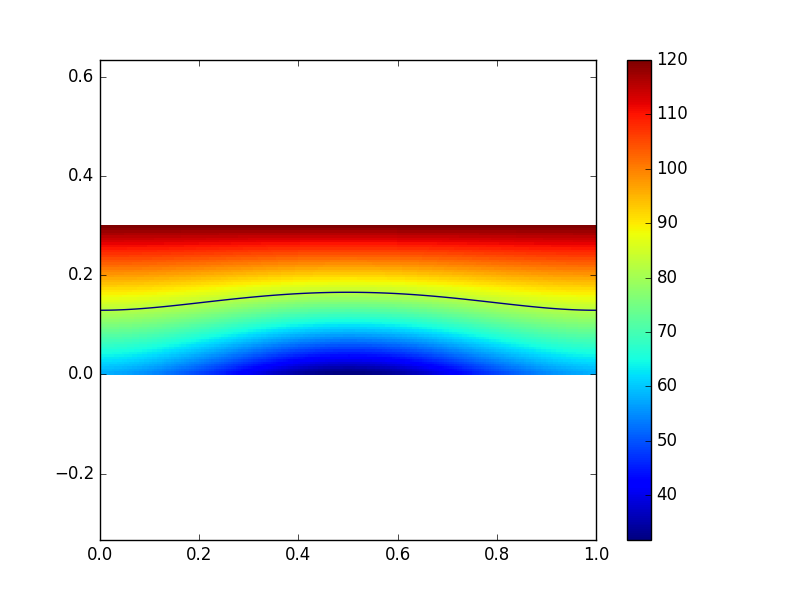
\includegraphics[width=0.7\textwidth]{pseudoColorPlot.png}
    \caption{Pseudocolor plot and mean temperature isoline for the 
    final solution given \textit{input2.txt}.}
    \label{Fig: viz-plot}
\end{figure}

\begin{thebibliography}{99}
\bibitem{projectpt1}
Software Development for Scientists and Engineers (2021), 
\emph{CME 211: Project Part 1}, Stanford University.
\bibitem{projectpt2}
Software Development for Scientists and Engineers (2021), 
\emph{CME 211: Project Part 2}, Stanford University.

\end{thebibliography}

\end{document}
